\documentclass[12pt]{article}

\usepackage{scicite,times,graphicx,float,hyperref}
\usepackage[skip=0pt]{caption}
\usepackage[utf8]{inputenc}
\usepackage{enumitem}
\usepackage{booktabs}

%%%%%%%%%%%%%%%%%%%%%%%%%%%%%%%%%%%%%%%%%%%%%%%%%%%%%%%%%%%%%%%%%%%%%%%%%%% PREAMBLE %%%%%%%%%%%%%%%%%%%%%%%%%%%%%%%%%%%%%%%%%%%%%%%%%%%%%%%%%%%%%%%%%%%%%%%%%%%

\topmargin -1.0cm
\oddsidemargin 0.0cm 
\textwidth 16cm 
\textheight 23cm
\footskip 1.0cm

\newenvironment{sciabstract}{%
\begin{quote} \bf}
{\end{quote}}

\newcounter{lastnote}
\newenvironment{scilastnote}{%
  \setcounter{lastnote}{\value{enumiv}}%
  \addtocounter{lastnote}{+1}%
  \begin{list}%
  {\arabic{lastnote}.}
  {\setlength{\leftmargin}{.22in}}
  {\setlength{\labelsep}{.5em}}
}
{\end{list}}

\title{Intermediate Report on:\\Pretix Cluster Deployment \& Management} 

\author
{Filipe Pires [85122], João Alegria [85048]\\
\\
Computational Infrastructures Management\\
\normalsize{Department of Electronics, Telecommunications and Informatics}\\
\normalsize{University of Aveiro}\\
} 

\date{\today{}}

%%%%%%%%%%%%%%%%%%%%%%%%%%%%%%%%%%%%%%%%%%%%%%%%%%%%%%%%%%%%%%%%%%%%%%%%%%%% REPORT %%%%%%%%%%%%%%%%%%%%%%%%%%%%%%%%%%%%%%%%%%%%%%%%%%%%%%%%%%%%%%%%%%%%%%%%%%%%

\begin{document} 

\baselineskip18pt

\maketitle 

\section*{Introduction} \label{introduction} %%%%%%%%%%%%%%%%%%%%%%%%%%%%%%%%%%%%%%%%%%%%%%%%%%%%%%%%%%%%%%%%%%%%%%%%%%%%%%%%%%%%%%%%%%%%%%%%%%%%%%%%%%%%%%%%%%%

This report aims to describe the work developed for the intermediate phase of the practical assignment of the discipline of Computational Infrastructures 
Management \cite{assign} from the Msc. degree in Informatics Engineering of the University of Aveiro at the Department of Electronics, Telecommunications and 
Informatics.
It is here included:
a product description and the respective expectations regarding client capacity, derived from a thorough analysis;
the adopted clustering strategy, considering matters such as virtualization, storage, network and load distribution mechanisms;
an explanation of the performance analysis executed based on the department's support platform for representative use cases;
and the results drawn from such analysis, to be considered during the second phase of development.

The service provided is Pretix, an online shop, box office and ticket outlet already successfully used by other service providers for conferences, festivals, 
exhibitions, workshops and more.
All code developed is publicly accessible in our GitHub repository:

\url{https://github.com/FilipePires98/GIC}.

\newpage
\section{Pretix Ticketing Software} \label{pretix} %%%%%%%%%%%%%%%%%%%%%%%%%%%%%%%%%%%%%%%%%%%%%%%%%%%%%%%%%%%%%%%%%%%%%%%%%%%%%%%%%%%%%%%%%%%%%%%%%%%%%%%%%%%%%

% what is pretix?

Pretix \cite{pretix} is an all-in-one product, serving as an online shop, box office and ticket outlet, meant for companies that aim to host events of numerous kinds.
This ticketing software created by Rami.io \cite{rami.io} has a wide variety of features that range from ticket shop customization (domain definition, multiple 
language support, product structure with multiple categories, packages and possibility for donations, seating plans, website embeddings, etc.) and marketing 
(voucher system, email, campaign tracking, etc.), to payment definition (invoicing and multiple payment methods) and on-site management (check-in lists, ticket 
scans, etc.), and even administrative control (with statistics and event-spanning reports, team permissions and data export and API).

As a complete solution, Pretix has already been successfully used for conferences, festivals, concerts, shows, exhibitions, workshops, barcamps, and more 
according to the creators.
The software's source code is completely open \cite{pretixgit}, and the authors make available extensive documentation \cite{pretixdoc}, an installation 
guide and a support blog.

\subsection{Our Product} \label{pretix.product} %%%%%%%%%%%%%%%%%%%%%%%%%%%%

% what is our purpose? what are we offering?

What we offer, as a developers team, is the Pretix' infrastructure deployment and management as a service that could potentially be provided to businesses 
interested in hosting events by taking advantage of Pretix' many advantages, without having resources or knowledge of how to deploy it themselves.
Our contract is simply to ensure the correct, reliable, secure and constant functioning of Pretix, capable of supporting usage scenarios of the same magnitude 
as of the one described next.

\subsection{Use Case Scenario} \label{pretix.scenario} %%%%%%%%%%%%%%%%%%%%%

% what do we intend to be able to support?
% how many users and/or requests per second is the system supposed to be able to handle?

In order to ensure the fulfillment of our contract, a representative scenario of usage was defined to guide us throughout development.
A simulated organization intends to host a WebSummit-like event by the end of this year.
It has analysed the feature list of Pretix and wishes to adopt it in the future.
However, as it is its first time using the software, the company decided to use it simply as a ticket purchase platform and reduced the payment methods to 
on-site manual payment only. 
The organization expects to sell 10 000 tickets in a week and warned us that in previous events they witnessed a peak close to the end of the selling period.

In practical terms this means that we only need to concern ourselves with the online ticket purchasing features and do not even need to consider the actual 
payment process, although it was our intent from the beginning to support most of Pretix's features even if most would not be used.
It also means that we had to build the system considering our hardware limitations and the activity peak expectation.

\subsection{Support Requirements} \label{pretix.requirements} %%%%%%%%%%%%%%

% what components need to exist for the product to be fully supported?
% what are the minimal hardware requirements for its deployment?

As stated in their documentation, to use Pretix it is required:
\vspace{-10pt}
\begin{itemize}[noitemsep]
  \item Pretix and the python packages it depends on
  \item An WSGI application server
  \item A periodic task runner
  \item A database
  \item A reverse proxy
  \item A server for caching, session storage and task queuing
\end{itemize}
\vspace{-10pt}
As we intended to deploy the product in containers, Docker became an additional requirement.

Regarding the hardware remotely available at our department, it was allocated for us an infrastructure of a total of 58 nodes and 115 cores, with 5.6TB of 
storage and 235.8GB of RAM available.
However, this is destined for several developer teams, meaning that we must only use a small portion of such resources, by our estimates of less than 10\% of 
the total capacity.

Also according to Pretix' documentation, the software has some scalability limitations.
In some cases their software needs to "fall back to event-global locking for some actions which are likely to run with high concurrency and cause harm".
For every event, only one of such locking actions can be run at the same time.
With this in mind, they estimate a maximum capacity of approximately 500 orders per minute per event, "even if you add more hardware".
However, they also mention that if the event to be hosted has an unlimited number of tickets (which is our case), fewer locking is applied and thus it is 
possible to reach approximately 1500 orders per minute per event.

Considering all of these aspects, we made an estimation of how many ticket purchase requests we would be able to support per minute.
At this preliminary stage, we believed it could be achieved a capacity of 800 ticket purchases per minute without a relevant amount of failed attempts.
In chapter \ref{performance} we explore our own system in an attempt to determine whether our estimations were correct and feasible or not.

%\texttt{java -cp <userdir>/build/classes fi.FarmInfrastructure}

% \vspace{-10pt}
% \begin{itemize}[noitemsep]
%   \item ...
% \end{itemize}
% \vspace{-10pt}

% \vspace{-10pt}
% \begin{enumerate}[noitemsep]
%   \item ...
% \end{enumerate}
% \vspace{-10pt}

% \begin{figure}[H]
%   \centering
%   \begin{minipage}{\textwidth}
%     \centering
%     \includegraphics[width=\linewidth]{img/.....png}
%   \end{minipage}%
%   \caption{...}
%   \label{...}
% \end{figure} 

\newpage
\section{Clustering Strategy} \label{strategy} %%%%%%%%%%%%%%%%%%%%%%%%%%%%%%%%%%%%%%%%%%%%%%%%%%%%%%%%%%%%%%%%%%%%%%%%%%%%%%%%%%%%%%%%%%%%%%%%%%%%%%%%%%%%%%%%%

\subsection{Architecture} \label{strategy.architecture} %%%%%%%%%%%%%%%%%%%% 

% what are the dependencies? what components does the cluster have?

Docker \cite{docker} allows us to deliver the infrastructure in isolated containers with well-defined communication channels.
This dramatically reduces infrastructure resources required and facilitates its management, while ensuring consistency within the whole environment.
Also, its simplicity in configurations and rapid deployment makes it perfect for its use in any system with a reasonably large size and complexity.

By taking advantage of Pretix' support for Docker, its dependencies were covered after analyzing which technologies would be most appropriate for our scenario.
With an already fully functional Docker Image publicly available \cite{pretix_img}, the authors of the product made the deployment of the web application easier.
In it is the Django-based \cite{django} web application that provides all the services and resources of Pretix, an instance of Gunicorn \cite{gunicorn}, a 
Web Server Gateway Interface (WSGI) hosting the application, and lastly an instance of NGinX \cite{nginx}, a reverse-proxy for the web application deployment 
in production mode - this last component is needed because the Django framework, when in production, divides the static resources and the dynamic resources and 
worries only about the dynamic ones, assuming that a reverse-proxy serves de static ones. 
Pretix' container configuration file also simplified the connection between the product and the storage containers, namely for the required database and caching server.

To handle all storage we chose PostgreSQL \cite{postgresql}.
This relational Database Management System (DBMS) had powerful tools to deal with scalability and redundancy, so it was quickly understood as a good option, 
although others like MariaDB were strongly considered as well.
It is the PostgreSQL that stores the data related to organizations, events, tickets, clients, invoices, etc.
In our case a PostgreSQL cluster is instantiated for redundancy purposes in a Master-Slave mode.
Currently, a single PostgreSQL master and 2 slave nodes are instantiated, and if the master fails the system is capable of assigning one of the slaves as the 
new master.

A similar approach was followed for the caching server.
This server has the responsibility of storing in-memory relevant data such as open user sessions, live events, etc. and of asynchronously queuing tasks.
In this case, the chosen tool was Redis \cite{redis}, instantiated in a Master-Slave cluster mode with 1 master and 2 slave nodes as well. 
The failover process is also supported with the help of sentinels. 
Sentinels are nodes natively supported by redis which have the responsibility of over-watching / taking care of the cluster and in case any change occurs, 
such as the addition or removal of a (slave or master) node, it registers that modification and notifies the necessary nodes so that they can reconfigure themselves. 
In our case we opted to instantiate two sentinels. \\

A problem encountered during the infrastructure configuration was that if a master node crashed in one of the storage clusters, the connection to the storage 
infrastructure was lost since the association to the cluster is through it's master(s).
With the master machine down in a distributed environment, the service was incapable of locating the new master. 
This and the efforts applied in balancing the load to the service forced us to add a proxy for both clusters.

Pgpool \cite{pgpool} was introduced to solve the problem for the PostgreSQL cluster. 
This middleware works between PostgreSQL servers and clients and enables connection pooling, replication, load balancing and more, although we used only the first
3 features.
This component served as a proxy that, when connected to, always redirects requests to the master of the PostgreSQL cluster and, if there was more than 1 master, 
the requests would be distributed in a balanced way over the available masters. 

For the Redis cluster, an HAProxy \cite{haproxy} was found to be the best option for our scenario, since it provided us a reliable and high performing load balancer.
This component, similarly to the one mentioned above, works as a proxy that forwards requests to one of the cluster masters, balancing the load in case there 
are severel master nodes.

The last component of our architecture is a reverse-proxy of our own, implemented using NginX, with the aim to balance the requests made to the Pretix service itself. 
This component, as suggested by the name reverse-proxy, also enabled us to access multiple instances of the Pretix server through a unique endpoint, facilitating 
the interaction between clients and service.

\begin{figure}[H]
  \centering
  \begin{minipage}{.85\textwidth}
    \centering
    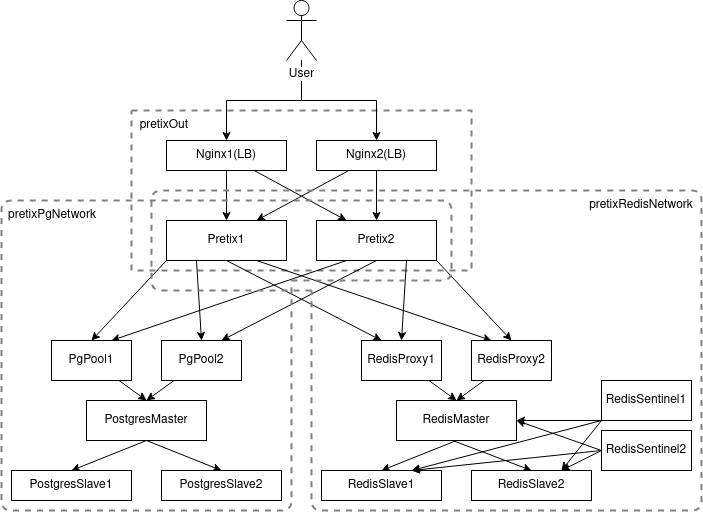
\includegraphics[width=\linewidth]{diagrams/InfrastructureArchitecture.png}
  \end{minipage}%
  \caption{Infrastructure architecture diagram deployed in Docker Swarm.}
  \label{fig:InfrastructureArchitecture}
\end{figure}

To provide this service we focused on some aspects that we considered paramount: availability, consistency, maintainability, scalability, redundancy, fault 
tolerance and load balancing. 
Those were the quality attributes we were looking to achieve when making every service redundant (by having replicas or through clusters), and when implementing 
the storage infrastructures as clusters and the mentioned proxies (for the storage systems and the service itself).
The result is visible in Figure \ref{fig:InfrastructureArchitecture}.

\subsection{Deployment} \label{strategy.deployment} %%%%%%%%%%%%%%%%%%%%%%%%

% how exactly is the system being deployed?

For this project there are 2 methods available to deploy the service stack: in a traditional Docker deployment through the usage of Docker Compose or in Docker 
Swarm mode.
The intended method was the second one, since the powerful infrastructure hosted in the DETI's department was made available for all groups. 
However, it was implemented not only a stack deployment for Docker Swarm but also one for the normal Docker Compose, since the second could be used for testing 
purposes. 
Both implementations respect our architecture but are naturally deployed with some differences in configurations, since each mode supports different features.

An experimentation phase occurred when searching for the best available solutions and containers that would suit our needs.
This in itself was quite a challenge, but the integration process of all containers proved to be far more challenging and complex than previously presumed.
The final version uses the following images from Docker Hub:
\vspace{-10pt}
\begin{itemize} [noitemsep]
  \item PostgreSQL Master/Slave: \href{https://hub.docker.com/r/bitnami/postgresql-repmgr}{https://hub.docker.com/r/bitnami/postgresql-repmgr}
  \item PostgreSQL Pool(PgPool): \href{https://hub.docker.com/r/bitnami/pgpool}{https://hub.docker.com/r/bitnami/pgpool}
  \item Redis Master/Slave/Sentinel: \href{https://hub.docker.com/\_/redis}{https://hub.docker.com/\_/redis}
  \item Redis Proxy: \href{https://hub.docker.com/\_/haproxy}{https://hub.docker.com/\_/haproxy}
  \item Pretix: \href{https://hub.docker.com/r/pretix/standalone}{https://hub.docker.com/r/pretix/standalone}
  \item NginX: \href{https://hub.docker.com/\_/nginx}{https://hub.docker.com/\_/nginx}
\end{itemize}
\vspace{-10pt}
Obviously, some of these images serve only as a base for self created images. 
This was desirable because in certain situations we needed a higher degree of control (e.g. for a container to wait for other containers to start first). 
This necessity for self-created images happened with: the Redis Slave image, to configure the Redis server to be a slave of a given machine and wait for the 
cluster master; the Redis Sentinel, to configure the Redis server to behave as a sentinel of the cluster and wait for the cluster master; the Redis Proxy, to 
configure the HAProxy so that the proxy would have in consideration all redis nodes and always access the master; and with Pretix itself, for the container 
to wait for the PostgreSQL and the Redis Proxies.

With each component defined, the stack was divided logically in 3 networks: each cluster belongs to one of the networks, NGinX has its own network, and the 
Pretix service is the linking element between the 3 networks.
This is also represented in Figure \ref{fig:InfrastructureArchitecture}.

Another aspect that we took in consideration was the data produced by the application itself. 
We needed a consistent and fault-tolerant system, so the data produced could not be lost under no circumstances. 
So volumes were assigned to the containers so that no information was lost, even if all services crashed.
All volumes were defined and mounted in a Network File System (NFS) provided \textit{a priori} for the discipline.

Lastly, some configuration files needed to be injected into containers, namely the Pretix server and the NginX reverse-proxy. 
To do this, we resort to the so called secrets: in our stack definition file, those configuration files were defined as secrets along with their destinations; 
such secrets are then generated automatically when the stack is deployed. 

Both Docker Compose and Docker Swarm accept the same stack configuration file. 
This is quite useful as it avoided duplicated work.
Nevertheless, as we have mentioned, there are significant differences between the 2 deployment methods, that in practical terms translates to certain fields 
being present in a mode and not in the other, namely the \texttt{deploy}, \texttt{configs} and \texttt{secrets} fields that are not processed in the Compose mode.
This meant that the automatic replication provided by Swarm is not available as well as the inject of configuration files and secret files. 
And since we mostly debugged and tested locally with Docker Compose, we felt the need to create an auxiliary stack configuration file that would deploy the 
system that replicates the one in Swarm (except for the NginX replication). 
In this file, the only changes were: the mounting point for the volumes (as this configuration was not intended to be deploy in the remote infrastructure); the 
replication (manually defined by creating different containers); and the configuration files otherwise injected by secrets API (now injected as volumes).

\subsection{Distribution} \label{strategy.distribution} %%%%%%%%%%%%%%%%%%%%

% how exactly is the system being distributed?

Docker Swarm not only adds some quite important features in the quality assuring realm (replication, load balancing, etc.), but it does that in a distributed way. 
This allows the Swarm mode to spread across as many machines as the user wants. 
The provided remote infrastructure is spread across 3 machines, each with several virtual machines created so that the swarm has more agents to use and thus 
simulating a truly heterogeneous and distributed environment.

Because we deploy our service stack in the Docker Swarm established in the remote infrastructure, our stack was distributed by design, which was one of the 
characteristics that appealed us in the beginning. 
This basically means that independently of the available machines, the number of machines, the machines' operational system, the location of the machine, and so on, installing docker on all of them and establishing the Swarm mode across all of them, we can safely guarantee that our stack can be deploy in that scenario and it will work as well as in the current one.

Through the usage of the provided platform, we concluded that the distribution is made automatically by assigning a task to an agent. A task is normally a replica of a service and the agent is a machine running a docker daemon somewhere in the Swarm network. Since each service consists in one or more replicas, they are spread across the Swarm network as the platform finds fit.

This distribution is quite important since it enables the user to gain access to the power of not only one machine, but all assigned to tasks of his stack, making possible smaller response times. This does not happen when a local deployment with Docker Compose is made, since this approach uses only one machine for all services needed, overloading all computational resources and possibly increasing the response times since the machine is worker more when compared to the ones in Swarm mode.

\newpage
\section{Current Cluster Performance} \label{performance} %%%%%%%%%%%%%%%%%%%%%%%%%%%%%%%%%%%%%%%%%%%%%%%%%%%%%%%%%%%%%%%%%%%%%%%%%%%%%%%%%%%%%%%%%%%%%%%%%%%%%%

% what was done to evaluate its current performance?

In order to determine the true capacity of our deployed solutions, a set of measures were performed both locally and on the remote, shared and more powerful 
infrastructure.
Although replication and redundancy were already concerns of ours, we were not yet focused on determining availability statistics.
Rather, our aim was to test our services in terms of load capacity.

We wished to determine how many users were supported simultaneously accessing Pretix and attempting to purchase tickets to our fictitious event.
To do this, we performed benchmarking tests and tracked the number of failures both in the act of requesting a purchase and in the act of storing purchases in 
our databases.
In this chapter we describe the efforts made for benchmarking and the bottlenecks discovered from our performance evaluation.

\subsection{Benchmarking} \label{performance.benchmarking} %%%%%%%%%%%%%%%%%

% what framework was used for load testing and how was it used?

After doing research on available tools and frameworks, we reached the conclusion that the most adequate would be Locust \cite{locust}.
Locust is an open source, intuitive, distributed, user load testing framework intended to "figure out how many concurrent users a system can handle" by 
programmatically simulating thousands of users called locusts.
During tests, systems are "attacked" by a swarm of locusts whose behavior is defined by the developer in Python and the swarming process is monitored from a 
web UI in real-time. 

When defining the behavior of our locusts, some considerations had to be dealt with.
The job of a locust wasn't simply to send an HTTP request to purchase a ticket; real users need to go through a purchasing process on Pretix' web platform, and 
in that process the user's browser requests far more data from the server than the mere purchase action.
So this process needed to be somehow simulated as well.
Several possibilities were considered to achieve this.

Selenium \cite{selenium}, a suite of tools for automating web browsers, is a widely used solution for testing purposes; however, we intended to launch thousands 
of virtual users and so, even with options such as launching browsers in headless mode (without rendering page elements), this created a bottleneck of processing 
elements that were not relevant to us and did not represent the true capacity of the system, thus rendering the whole benchmark invalid.
Other alternatives like wrappers to drive browsers in Python were tried but proved to be too limited for our purposes.

The solution was to manually go through the purchase process once on the Pretix website and collect all network requests that were being made, including CSS 
resources, image files, Javascript code and requests sent to Pretix' REST API.
Amongst these requests was the actual purchase action in a message of type POST.
Then, we replicated all requests on the locust behavior and, by reading Pretix' API documentation, were able to manipulate the POST request to seem to come 
from different users.
We also included optional data on such requests, like invoices, to increase the load the server needed to process and so establishing a worst-case-scenario usage 
that would give us more comfort regarding the faithfulness of the results.

\subsection{Execution} \label{performance.execution} %%%%%%%%%%%%%%%%%%%%%%%

% how was the benchmarking done?

Having established the behavior of the fictitious users, we proceeded to actually executing our benchmarking.
This was divided in 2 groups of tests of 4 phases each.
The first group was entirely performed locally in one of our personal computers, the second was performed remotely using our Docker Swarm.
This was done in order to clearly comprehend the differences of performance between the 2 deployment methods and detect which bottlenecks were common to both, 
which were surpassed with greater hardware capacity and which appeared only in the second group (if any).

The 4 phases consisted in load testing the solution with 4 different activity peaks: one with half the expected load, one with the expected load, one with 
twice as many expected users and one with 10 times as many users.
These were defined a priori and the expected load was set according to the analysis described in section \ref{pretix.requirements}. 

It is important to mention that some failed requests were treated in a particular manner after reflecting on the issue.
This is the case for accessing requests to the ticket purchase root path and for completing a purchase process.
In these situations the fictitious user attempts to successfully execute them 3 times.
This was decided after considering that in reality, an interested client would not mind to have to reload a page in the event it failed the first time, even more 
if this would occur in the completing action of the ticket purchase.
Although this naturally improved the results, all failures were considered in our overall evaluation.
Failures are here distinguished from 3-times failures by naming the later as exceptions. \\

The results of the first group of tests are presented next.
For the local tests it is important to consider the hardware used and its activity in stand-by.
It was used a computer with 12Gb of RAM and 8 CPU cores; before any tests were executed, 1 thread was running with CPU at 10\% of its capacity and around 6Gb 
of memory being used.

The first locust swarm attacked the service with 400 clients, with a hatch rate of 20 per second (the maximum rate found for the hardware to handle).
The attack took about 1 minute and 26 seconds, with the swarm complete 34 seconds after initialization.
... \\


%%%%%%%%%%%%%%%%%%%%%%%%%%%%%%%%%%%%%%%%

% https://docs.pretix.eu/en/latest/api/fundamentals.html
% Responses with status code 409 Conflict are not cached. If you send the request again, it will be executed as a new request, since these responses are intended to be retried.

%%%%%%%%%%%%%%%%%%%%%%%%%%%%%%%%%%%%%%%%

% 0
% 0/s

% Mem 7.4Gb / 11.6Gb
% 8 cores at ~10\%
% 1 thr running

%%%%%%%%%%%%%%%%%%%%%%%%%%%%%%%%%%%%%%%%

% 400
% 20/s

%  (start),  (all users),  (end)

% Mem 9.63Gb / 11.6Gb
% 8 cores at ~70\%
% 8 thr running

% Type 	Name 	                                        # Requests 	# Fails   # Exceptions  Median (ms) 	90%ile (ms) 	Average (ms) 	Min (ms) 	Max (ms) 	Average size (bytes)
% POST 	/api/v1/organizers/ws/events/ws2020/orders/ 	456 	      59 	      3             810 	        1500 	        1024 	        150 	    11199 	  1098
%       Aggregated                                    22435       59        -             610           990           737           3         50278     71693 

%%%%%%%%%%%%%%%%%%%%%%%%%%%%%%%%%%%%%%%%

% 800
% 20/s

%  (start),  (all users),  (end)

% Mem 9.87Gb / 11.6Gb
% 8 cores at ~70\%
% 8 thr running

% Type 	Name 	                                        # Requests 	# Fails   # Exceptions  Median (ms) 	90%ile (ms) 	Average (ms) 	Min (ms) 	Max (ms) 	Average size (bytes)
% POST 	/api/v1/organizers/ws/events/ws2020/orders/ 	906 	      109 	    3             1300 	        1800 	        1325 	        165 	    8682 	    1093
%       Aggregated                                    44885       369       -             1100          1700          1343          2         83344     71436

%%%%%%%%%%%%%%%%%%%%%%%%%%%%%%%%%%%%%%%%

% 1600
% 20/s

%  (start),  (all users),  (end)

% Mem 10.0Gb / 11.6Gb
% 8 cores at ~70\%
% 8 thr running

% Type 	Name 	                                        # Requests 	# Fails   # Exceptions  Median (ms) 	90%ile (ms) 	Average (ms) 	Min (ms) 	Max (ms) 	Average size (bytes)
% POST 	/api/v1/organizers/ws/events/ws2020/orders/ 	1772 	      178 	    6             1800 	        3200 	        2904 	        173 	    121762 	  1122
%       Aggregated 	                                  89730 	    1426 	    -             1400 	        3200 	        3232 	        2 	      181509 	  70780

%%%%%%%%%%%%%%%%%%%%%%%%%%%%%%%%%%%%%%%%

% 8000
% 20/s

%  (start),  (all users),  (end)

% Mem 10.8Gb / 11.6Gb
% 8 cores at ~70\%
% 8 thr running

% Type 	Name 	                                        # Requests 	# Fails   # Exceptions  Median (ms) 	90%ile (ms) 	Average (ms) 	Min (ms) 	Max (ms) 	Average size (bytes)
% POST 	/api/v1/organizers/ws/events/ws2020/orders/ 	9177 	      1214 	    37            2700 	        5000 	        15635 	      62 	      1022473 	995
%       Aggregated 	                                  448918 	    10898 	  -             1900 	        4600 	        20335 	      2 	      1579377 	70336

%%%%%%%%%%%%%%%%%%%%%%%%%%%%%%%%%%%%%%%%



With the system fully deployed using Docker Swarm, the second group of tests was executing, resulting in the following values.
... 

\subsection{Bottlenecks} \label{performance.bottlenecks} %%%%%%%%%%%%%%%%%%%

% what performance bottlenecks were found?

...

\newpage
\section{Additional Remarks} \label{remarks} %%%%%%%%%%%%%%%%%%%%%%%%%%%%%%%%%%%%%%%%%%%%%%%%%%%%%%%%%%%%%%%%%%%%%%%%%%%%%%%%%%%%%%%%%%%%%%%%%%%%%%%%%%%%%%%%%%%

\subsection{Pretix Quickstart} \label{remarks.quickstart} %%%%%%%%%%%%%%%%%%

% quickstart script

During development, a need for a faster basic setup of Pretix emerged for debugging purposes.
As many of our tests assumed the existence of organizers and events already inserted on the databases, each time these had to be cleared the objects had to be 
manually created before proceeding with some implementation process.

In order to respond to this need, we developed a Python script capable of completely dispose of the manual labour.
This script, which we called \texttt{quickstart.py} and placed under the scripts folder, uses Selenium \cite{selenium} to create an organization inside Pretix, 
generate a secret API key for sending REST requests (storing it in a text file), create a default event and prepare it for load testing with Locust.
It also contains configurable variables to personalize its output.

Such quickstart tool was not only found useful for the obvious advantage in development speed it brought to us, but was also considered a good help tool for any 
person that wishes to quickly experiment our infrastructure without having to know much about Pretix itself.

\subsection{Planning Phase 2} \label{remarks.planning} %%%%%%%%%%%%%%%%%%%%%

% what is to be done until the final delivery?
% docker secrets, fault tolerance, 

Although with a service stack already replicated, redundant and tolerant to failures, now that we have a better understanding of the service itself, it's bottlenecks and it's behavior when handling with higher volumes of data and incoming requests we can personalize and optimize the stack for Pretix itself. For that reason our concerns shifted towards making the solution more fault tolerant, scalable, reliable and in general more robust, taking advantage of the already obtained conclusions on what components limited our service and needed more attention.

A big aspect that we already considered, but was from the beginning destined to be tackled in the second and last delivery of this project is the handling of errors, crashes and traffic fluctuations. In practical terms this is translated in the development of automatic mechanisms that allows the infrastructure manager to be certain that a service will never fail or to quickly scale the service's stack according to incoming traffic. Some efforts related to this theme were already made on this first delivery, namely the implementation of clusters for both of the storage systems necessary for Pretix; our implementation of both clusters already guarantees replication and redundancy of information and tolerant to failures since any node can fail, redefining the cluster if necessary.

The proposed further work in this area is to develop Ansible scripts that will enable us to scale automatically our service stack and possibly handle automatically with service crashes and their respective redeployment. Ansible \cite{ansible} is a IT automation engine that automates cloud provisioning, configuration management, application deployment, intra-service orchestration, and many other IT needs, exactly the type of engine we needed to further improve our service infrastructure.

Some more questions will be taken in consideration, namely security. By injecting any password needed to services through the secrets Docker API we aim to achieve a more secure and penetration resistant system. This was already done with configuration files needed to be injected in some of our services, but we intend to extend this process to any critical information, such as passwords.


\subsection{Documentation} \label{remarks.documentation} %%%%%%%%%%%%%%%%%%%

% what documentation was produced?

A great portion of the code we deal with isn't of our authorship, so the documentation it contains is the documentation we get.
Nevertheless, the code we developed has specific purposes and, although usually very much self explanatory due to its nature, should be easy to interpret by any person.
Our goal is to ensure that what we deliver can be easily reused or even continued by other developers.

With this in mind, we made significant efforts on ensuring that all code developed by us followed a common structure with the same coding style.
Also, we made sure all source files have a description of their purpose and relevant information on the first lines, and contain comments on key points of the 
code explaining snippets considered of greater complexity/importance.

\subsection{Assignment Contributions} \label{remarks.contributions} %%%%%%%%

% who did what?

Regarding the work distribution amongst developers, a close-contact strategy was defined where each worked on a cluster component or piece of software according 
to a predefined plan. 
The cluster strategy and respective details were decided in conjunction, as well as the key objectives and tasks to be achieved before the final delivery deadline.

Pretix' features were explored by both developers in order to better comprehend the web platform and the REST API.
Then, João focused on the deployment of our solution on the department's infrastructure while Filipe focused on creating and executing the load tests.
The analysis of the results were carefully conducted in conjunction as well, in order to maintain a common knowledge for better workflows.
It is needless to say that bug and error solving was made along the development phase by both developers any time it was required.

Once performance benchmarking and bottleneck identification were completed, this report and the code documentation became our primary concern, with both 
contributing equally.

\newpage
\section*{Conclusions} \label{conclusions} %%%%%%%%%%%%%%%%%%%%%%%%%%%%%%%%%%%%%%%%%%%%%%%%%%%%%%%%%%%%%%%%%%%%%%%%%%%%%%%%%%%%%%%%%%%%%%%%%%%%%%%%%%%%%%%%%%%%%

...

\begin{thebibliography}{9} %%%%%%%%%%%%%%%%%%%%%%%%%%%%%%%%%%%%%%%%%%%%%%%%%%%%%%%%%%%%%%%%%%%%%%%%%%%%%%%%%%%%%%%%%%%%%%%%%%%%%%%%%%%%%%%%%%%%%%%%%%%%%%%%%%%%%
  \bibliographystyle{Science}

  \bibitem{assign}
    J. P. Barraca,
    \textit{GIC - Report no.1: Simple Product Operation},
    University of Aveiro,
    2019/20.
    \vspace{-10pt}

  \bibitem{pretix}
    \textit{About Pretix},
    \url{https://pretix.eu/about/en/}.
    Pretix.eu,
    retrieved in April 2020.
    \vspace{-10pt}

  \bibitem{rami.io}
    \textit{Welcome to Rami.io},
    \url{https://rami.io/}.
    Rami.io,
    retrieved in April 2020.
    \vspace{-10pt}

  \bibitem{pretixgit}
    \textit{Pretix Code Repository},
    \url{https://github.com/pretix/pretix}.
    GitHub, Inc.,
    retrieved in April 2020.
    \vspace{-10pt}

  \bibitem{pretixdoc}
    \textit{Welcome to pretix' documentation!},
    \url{https://docs.pretix.eu/en/latest/}.
    Pretix.eu,
    retrieved in April 2020.
    \vspace{-10pt}

  \bibitem{docker}
    \textit{Docker Homepage},
    \url{https://www.docker.com/}.
    Docker Inc.,
    retrieved in April 2020.
    \vspace{-26pt}

  \bibitem{pretix_img}
    \textit{pretix/standalone},
    \url{https://hub.docker.com/r/pretix/standalone}.
    pretix,
    retrieved in April 2020.
    \vspace{-10pt}

  \bibitem{django}
    \textit{Meet Django},
    \url{https://www.djangoproject.com/}.
    Django Software Foundation and individual contributors,
    retrieved in April 2020.
    \vspace{-10pt}

  \bibitem{gunicorn}
    \textit{Gunicorn Homepage},
    \url{https://gunicorn.org/}.
    Gunicorn.org,
    retrieved in April 2020.
    \vspace{-10pt}

  \bibitem{nginx}
    \textit{NGinX News},
    \url{https://nginx.org/}.
    NGinX.org,
    retrieved in April 2020.
    \vspace{-10pt}

  \bibitem{postgresql}
    \textit{PostgreSQL: The World's Most Advanced Open Source Relational Database},
    \url{https://www.postgresql.org/}.
    The PostgreSQL Global Development Group,
    retrieved in April 2020.
    \vspace{-10pt}

  \bibitem{redis}
    \textit{About Redis},
    \url{https://redis.io/}.
    Redis Labs,
    retrieved in April 2020.
    \vspace{-10pt}

  \bibitem{pgpool}
    \textit{Welcome to Pgpool-II},
    \url{https://www.pgpool.net/mediawiki/index.php/Main_Page}.
    PgPool Global Development Group,
    retrieved in April 2020.
    \vspace{-10pt}

  \bibitem{haproxy}
    \textit{HAProxy: The Reliable, High Performance TCP/HTTP Load Balancer},
    \url{https://www.haproxy.org/}.
    HAProxy.org,
    retrieved in April 2020.
    \vspace{-10pt}

  

  \bibitem{locust}
    \textit{Locust, an open source load testing tool},
    \url{https://locust.io/}.
    Locust.io,
    retrieved in April 2020.
    \vspace{-10pt}

  \bibitem{selenium}
    \textit{About Selenium},
    \url{https://www.selenium.dev/about/}.
    Software Freedom Conservancy,
    retrieved in April 2020.
    \vspace{-10pt}

  \bibitem{ansible}
    \textit{Ansible},
    \url{https://www.ansible.com/}.
    Red Hat,
    retrieved in April 2020.
    

\end{thebibliography}

\clearpage

\end{document}




















